\documentclass[12pt]{article}

\usepackage[margin=1in]{geometry} 
\usepackage{amsmath,amsthm,amssymb,scrextend}
\usepackage{fancyhdr}
\pagestyle{fancy}
\usepackage{xcolor}
\usepackage{pgfplots}
\usepackage{enumitem}
\pgfplotsset{compat=1.18}

\newcommand{\N}{\mathbb{N}}
\newcommand{\Z}{\mathbb{Z}}
\newcommand{\I}{\mathbb{I}}
\newcommand{\R}{\mathbb{R}}
\newcommand{\Q}{\mathbb{Q}}
\renewcommand{\qed}{\hfill$\blacksquare$}
\let\newproof\proof
\renewenvironment{proof}{\begin{addmargin}[1em]{0em}\begin{newproof}}{\end{newproof}\end{addmargin}\qed}
% \newcommand{\expl}[1]{\text{\hfill[#1]}$}

\newenvironment{theorem}[2][Theorem]{\begin{trivlist}
		\item[\hskip \labelsep {\bfseries #1}\hskip \labelsep {\bfseries #2.}]}{\end{trivlist}}
\newenvironment{lemma}[2][Lemma]{\begin{trivlist}
		\item[\hskip \labelsep {\bfseries #1}\hskip \labelsep {\bfseries #2.}]}{\end{trivlist}}
\newenvironment{problem}[2][Problem]{\begin{trivlist}
		\item[\hskip \labelsep {\bfseries #1}\hskip \labelsep {\bfseries #2.}]}{\end{trivlist}}
\newenvironment{exercise}[2][Exercise]{\begin{trivlist}
		\item[\hskip \labelsep {\bfseries #1}\hskip \labelsep {\bfseries #2.}]}{\end{trivlist}}
\newenvironment{reflection}[2][Reflection]{\begin{trivlist}
		\item[\hskip \labelsep {\bfseries #1}\hskip \labelsep {\bfseries #2.}]}{\end{trivlist}}
\newenvironment{proposition}[2][Proposition]{\begin{trivlist}
		\item[\hskip \labelsep {\bfseries #1}\hskip \labelsep {\bfseries #2.}]}{\end{trivlist}}
\newenvironment{corollary}[2][Corollary]{\begin{trivlist}
		\item[\hskip \labelsep {\bfseries #1}\hskip \labelsep {\bfseries #2.}]}{\end{trivlist}}

\setlength{\parindent}{0pt}

\begin{document}
	% for only the first page and for all the pages for pdf version
	\fancyhf{}
	\lhead{Formulas}
	\section*{Some Taylor / Maclaurin  Series Formulas}

	\[\boldsymbol{f(x)} = \sum_{n=0}^{\infty} \frac{f^{(n)}(a)}{n!}(x-a)^n = f(a) + f'(a)(x-a) + \frac{f''(a)}{2!}(x-a)^2 + \cdots\]

	When $a=0$, it is Maclaurin series:

	\[\boldsymbol{f(x)} = \sum_{n=0}^{\infty} \frac{f^{(n)}(0)}{n!}x^n = f(0) + f'(0)x + \frac{f''(0)}{2!}x^2 + \frac{f'''(0)}{3!}x^3 + \cdots\]

	\[\begin{aligned}
		\boldsymbol{e^{x}}&=\sum_{n=0}^{\infty} \frac{1}{n !} x^{n}=1+x+\frac{1}{2 !} x^{2}+\cdots, \quad x \in(-\infty,+\infty) \\[1ex]
		\boldsymbol{\sin x}&=\sum_{n=0}^{\infty} \frac{(-1)^{n}}{(2 n+1) !} x^{2 n+1}=x-\frac{1}{3 !} x^{3}+\frac{1}{5 !} x^{5}+\cdots,\quad x \in(-\infty,+\infty) \\[1ex]
		\boldsymbol{\cos x}&=\sum_{n=0}^{\infty} \frac{(-1)^{n}}{(2 n) !} x^{2 n}=1-\frac{1}{2 !} x^{2}+\frac{1}{4 !} x^{4}+\cdots,\quad  x \in(-\infty,+\infty) \\[1ex]
		\boldsymbol{\ln (1+x)}&=\sum_{n=0}^{\infty} \frac{(-1)^{n}}{n+1} x^{n+1}=x-\frac{1}{2} x^{2}+\frac{1}{3} x^{3}+\cdots,\quad  x \in(-1,1] \\[1ex]
		\boldsymbol{\frac{1}{1-x}}&=\sum_{n=0}^{\infty} x^{n}=1+x+x^{2}+x^{3}+\cdots,\quad  x \in(-1,1) \\[1ex]
		\boldsymbol{\frac{1}{1+x}}&=\sum_{n=0}^{\infty}(-1)^{n} x^{n}=1-x+x^{2}-x^{3}+\cdots,\quad  x \in(-1,1)\\[1ex]
		\boldsymbol{(1+x)^{\alpha}}&=1+\sum_{n=1}^{\infty} \frac{\alpha(\alpha-1) \cdots(\alpha-n+1)}{n !} x^{n}=1+\alpha x+\frac{\alpha(\alpha-1)}{2 !} x^{2}+\cdots,\quad  x \in(-1,1) \\[1ex]
		\boldsymbol{\arctan x}&=\sum_{n=0}^{\infty} \frac{(-1)^{n}}{2 n+1} x^{2 n+1}=x-\frac{1}{3} x^{3}+\frac{1}{5} x^{5}+\cdots,\quad  x \in[-1,1] \\[1ex]
		\boldsymbol{\arcsin x}&=\sum_{n=0}^{\infty} \frac{(2 n) !}{4^{n}(n !)^{2}(2 n+1)} x^{2n+1}=x+\frac{1}{6} x^{3}+\frac{3}{40} x^{5}+\frac{5}{112} x^{7}+\frac{35}{1152} x^{9}+\cdots,\quad  x \in(-1,1)\\[1ex]
		\boldsymbol{\tan x}&=\sum_{n=1}^{\infty} \frac{B_{2 n}(-4)^{n}\left(1-4^{n}\right)}{(2 n) !} x^{2 n-1}=x+\frac{1}{3} x^{3}+\frac{2}{15} x^{5}+\frac{17}{315} x^{7}+\frac{62}{2835} x^{9}+\cdots,\quad x\in (-\frac{\pi}{2},\frac{\pi}{2})
	\end{aligned}\]
	\newpage

	\section*{Hyperbolic Trigonometric Identities}
	$$
	\sinh x = \frac{e^x - e^{-x}}{2}
	$$
	
	$$
	\cosh x = \frac{e^x + e^{-x}}{2}
	$$
	
	$$
	\tanh x = \frac{\sinh x}{\cosh x} = \frac{e^x - e^{-x}}{e^x + e^{-x}}
	$$

	\begin{center}
	\begin{tikzpicture}
	\begin{axis}[
		width=0.9\textwidth,
		height=0.32\textheight,
		xmin=-5, xmax=5,
		ymin=-3, ymax=3,
		axis lines=middle,
		xlabel={$x$},
		ylabel={$y$},
		ylabel style={at={(axis description cs:0.5,1.02)},anchor=south},
		xtick=\empty,
		ytick=\empty,
		xticklabels={},
		yticklabels={},
		axis equal image=true,
		legend style={at={(0.98,0.02)},anchor=south east,fill=white},
		samples=200
	]
	\addplot[red, thick] {sinh(x)};
	\addlegendentry{$\sinh x$}
	\addplot[blue, thick] {cosh(x)};
	\addlegendentry{$\cosh x$}
	\addplot[green!40!black, thick] {tanh(x)};
	\addlegendentry{$\tanh x$}
	\end{axis}
	\end{tikzpicture}
	\end{center}
	
	$$
	\coth x = \frac{\cosh x}{\sinh x} = \frac{e^x + e^{-x}}{e^x - e^{-x}}
	\qquad \text{for } x \ne 0
	$$
	
	$$
	\operatorname{sech} x = \frac{1}{\cosh x} = \frac{2}{e^x + e^{-x}}
	$$
	
	$$
	\operatorname{csch} x = \frac{1}{\sinh x} = \frac{2}{e^x - e^{-x}}
	\qquad \text{for } x \ne 0
	$$

	\begin{center}
	\begin{tikzpicture}
	\begin{axis}[
		width=0.9\textwidth,
		height=0.32\textheight,
		xmin=-5, xmax=5,
		ymin=-3, ymax=3,
		axis lines=middle,
		xlabel={$x$},
		ylabel={$y$},
		ylabel style={at={(ticklabel* cs:1.05)},anchor=center},
		xtick=\empty,
		ytick=\empty,
		xticklabels={},
		yticklabels={},
		axis equal image=true,
		legend style={at={(0.98,0.02)},anchor=south east,fill=white},
		samples=200
	]
	\addplot[red, thick, domain=-5:-0.08] {cosh(x)/sinh(x)};
	\addplot[red, thick, domain=0.08:5, forget plot] {cosh(x)/sinh(x)};
	\addlegendentry{$\coth x$}
	\addplot[blue, thick, domain=-5:5] {1/cosh(x)};
	\addlegendentry{$\operatorname{sech} x$}
	\addplot[green!40!black, thick, domain=-5:-0.08] {1/sinh(x)};
	\addplot[green!40!black, thick, domain=0.08:5, forget plot] {1/sinh(x)};
	\addlegendentry{$\operatorname{csch} x$}
	\end{axis}
	\end{tikzpicture}
	\end{center}
	
	\newpage

	\subsection*{Converting Product to Summation }
	$$
	S_n=\prod_{k=1}^{n} a_k \quad (a_k>0)
	$$
	
	$$
	\ln(S_n)=\sum_{k=1}^{n}\ln(a_k)
	$$
	
	Since \(\ln x\) is continuous on \((0,\infty)\),
	
	$$
	\ln\left(\prod_{k=1}^{\infty} a_k\right)
	=
	\ln\left(\lim_{n\to\infty}P_n\right)
	=
	\lim_{n\to\infty}\ln(P_n)
	$$
	
	According to logarithm rule:
	$$\ln(a_0\times a_1\times a_2\times \cdots\times a_n)=\ln(a_0)+\ln(a_1)+\ln(a_2)+\cdots+\ln(a_n)$$
	
	Thus, 
	$$
	\ln(S_n)=\ln\left(\prod_{k=1}^{n} a_k\right)=\sum_{k=1}^{n}\ln(a_k)
	$$
	
	

\end{document}
